\begin{figure}[htbp]
\centering
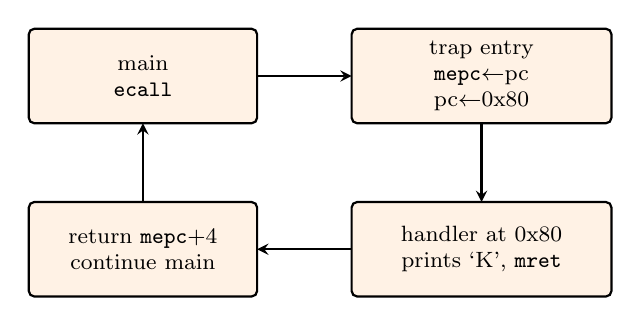
\begin{tikzpicture}[font=\footnotesize, >=stealth, x=1cm, y=1cm]
  \draw[thick, fill=orange!10, rounded corners=2pt] (0,2.6) rectangle (2.9,3.8);
  \node[align=center] at (1.45,3.2) {main\\ \texttt{ecall}};
  \draw[thick, fill=orange!10, rounded corners=2pt] (4.1,2.6) rectangle (7.4,3.8);
  \node[align=center] at (5.75,3.2) {trap entry\\ \texttt{mepc}$\leftarrow$pc\\ pc$\leftarrow$0x80};
  \draw[thick, fill=orange!10, rounded corners=2pt] (4.1,0.4) rectangle (7.4,1.6);
  \node[align=center] at (5.75,1.0) {handler at 0x80\\ prints `K', \texttt{mret}};
  \draw[thick, fill=orange!10, rounded corners=2pt] (0,0.4) rectangle (2.9,1.6);
  \node[align=center] at (1.45,1.0) {return \texttt{mepc}+4\\ continue main};
  \draw[->, thick] (2.9,3.2) -- (4.1,3.2);
  \draw[->, thick] (5.75,2.6) -- (5.75,1.6);
  \draw[->, thick] (4.1,1.0) -- (2.9,1.0);
  \draw[->, thick] (1.45,1.6) -- (1.45,2.6);
\end{tikzpicture}
\caption{The minimal trap path implemented in this chapter's core:
\texttt{ecall} saves the faulting pc in \texttt{mepc} and jumps to the
fixed vector 0x80; \texttt{mret} returns to \texttt{mepc}+4.}
\label{fig:trap08}
\end{figure}
